\chapter{Empirical priors: pancreatitis}
\label{applications-priors_empirical}

Moving away from more `subjective' expert priors, empirical priors
rely on the data.  Similar to fitting the complete hierarchical model,
empirical priors use predictions from a simple global model to inform
parallel regional models, as discussed in Chapter
\ref{theory-age_pattern_model}.  In modeling diseases with
_____________, such as pancreatitis, empirical priors provide data-derived
relationships to guide the modeling process.

Unless there are data to inform otherwise, the highest hierarchal level assumes the empirical prior is true.  In the case of pancreatitis, regional data

Pancreatitis is the inflammation of the pancreas, most commonly 
caused by alcohol or gallstones.  In most cases, the disease resolves 
itself and there is no need for treatment.  However, some acute 
cases develop pancreatic necrosis and systemic organ failure.  These 
complications require immediate treatment and have a high mortality risk. 
\cite{raraty_acute_2004, banks_epidemiology_2002, sekimoto_JPN_2006}

Data from systematic review yielded $3950$ incidence data points, $373$ of which 
are from Eastern Europe, the example in this chapter.  As shown in 
Figure~\ref{fig:app-pan data}, the data are very heterogeneous.

    \begin{figure}[h]
        \begin{center}
            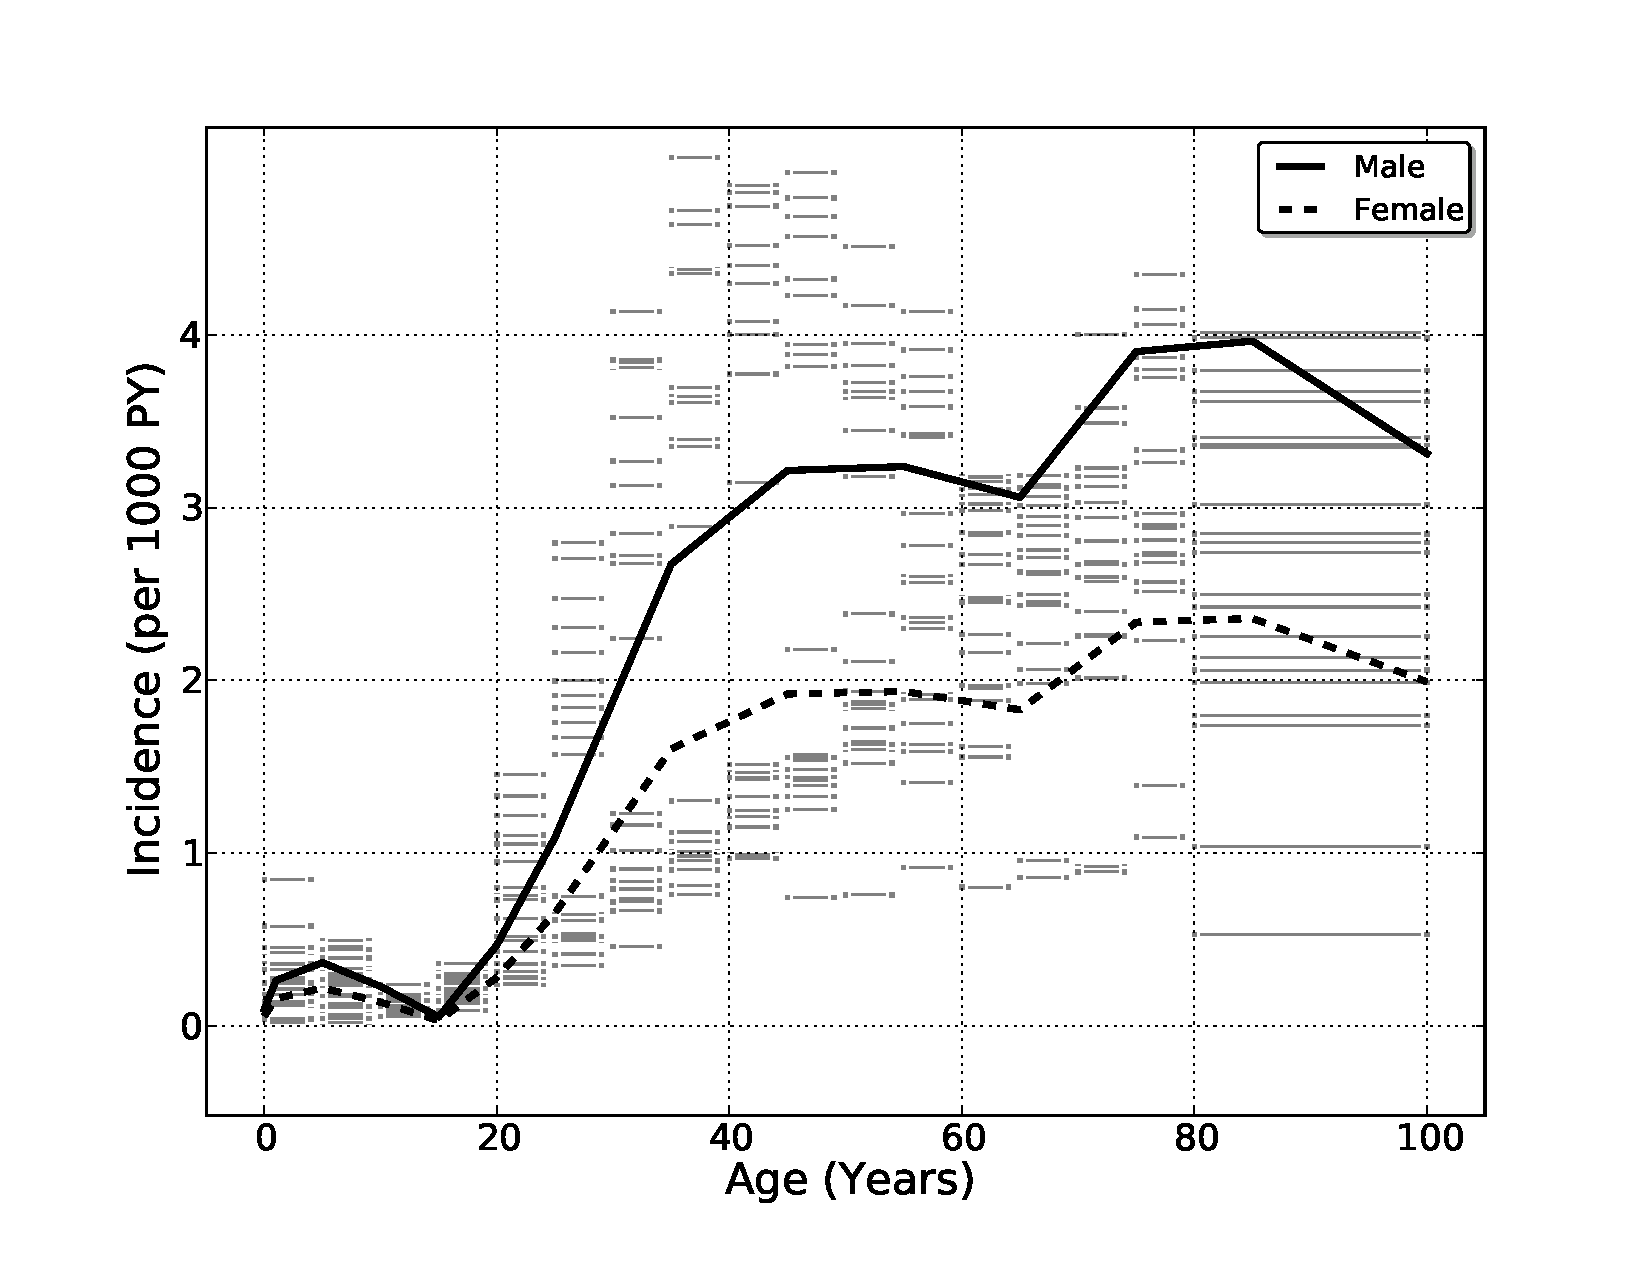
\includegraphics[width=\textwidth]{pancreatitis-data.pdf}
            \caption{Pancreatitis incidence estimates for males and females
              in Eastern Europe, 2005.}
            \label{fig:app-pan data}
        \end{center}
    \end{figure}

However, further investigation shows that the data heterogeneity is not 
random but the result of a sex differential.

    \begin{figure}[h]
        \begin{center}
            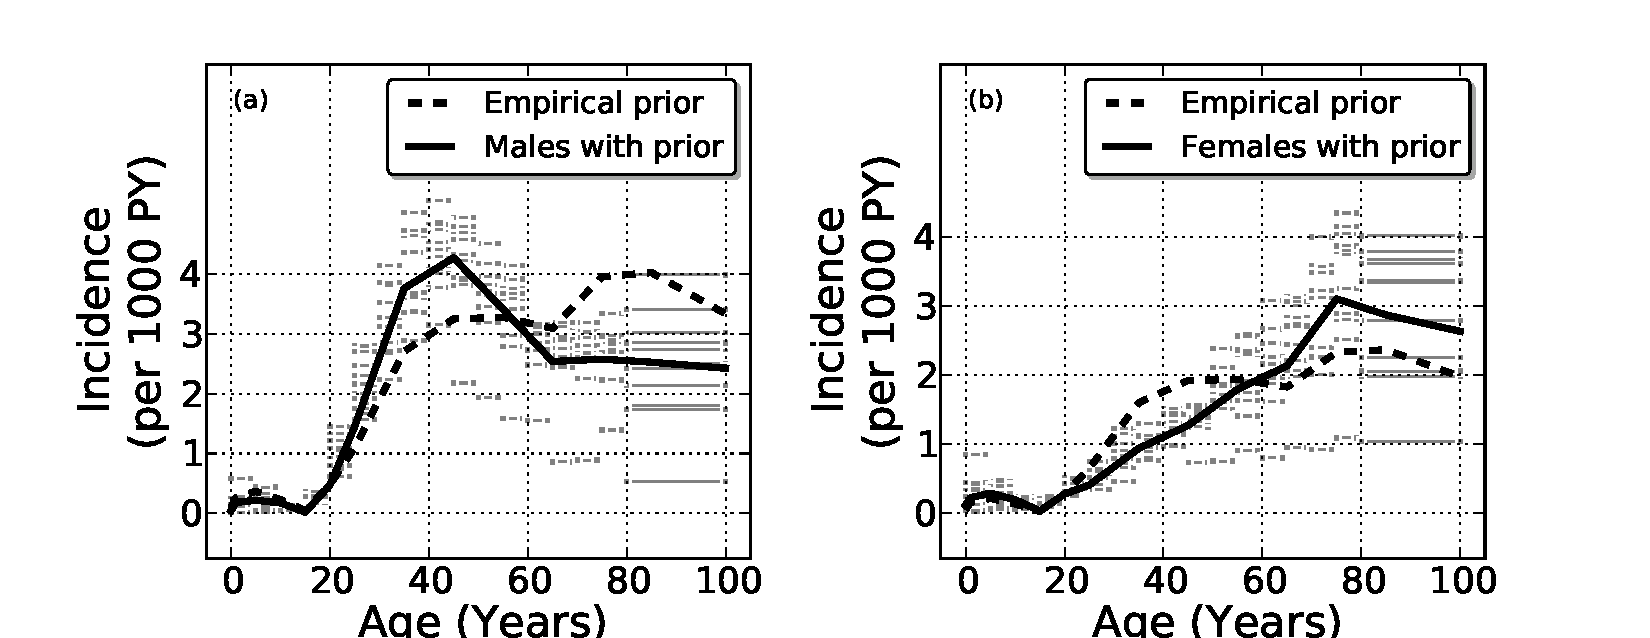
\includegraphics[width=\textwidth]{pancreatitis-compare.pdf}
            \caption{A comparison of incidence estimates for males (a) and 
              females (b) in Eastern Europe.}
            \label{fig:app-pan compare}
        \end{center}
    \end{figure}